\hypertarget{introduction}{%
\section{Introduction}\label{introduction}}

To complete this activity, I participated in CrowdStrike's annual
\href{https://www.crowdstrike.com/en-us/events/adversary-week/}{Adversary
Week}, an entirely online event where CrowdStrike's security experts
share insights into the current threat landscape through a series of
interactive seminars. The event, while open to everyone, is primarily
aimed at security defenders as it focuses on analysing modern
adversaries and identifying strategies to strengthen defence.

This year's event focused on the increased prominence of artificial
intelligence in cyberattacks, highlighting how AI is accelerating
adversary capabilities and increasing the complexity of modern defence
mechanisms. Topics covered by the seminars included cross-domain
attacks, ransomware attacks, identity-based attacks, and prompt
injection attacks. 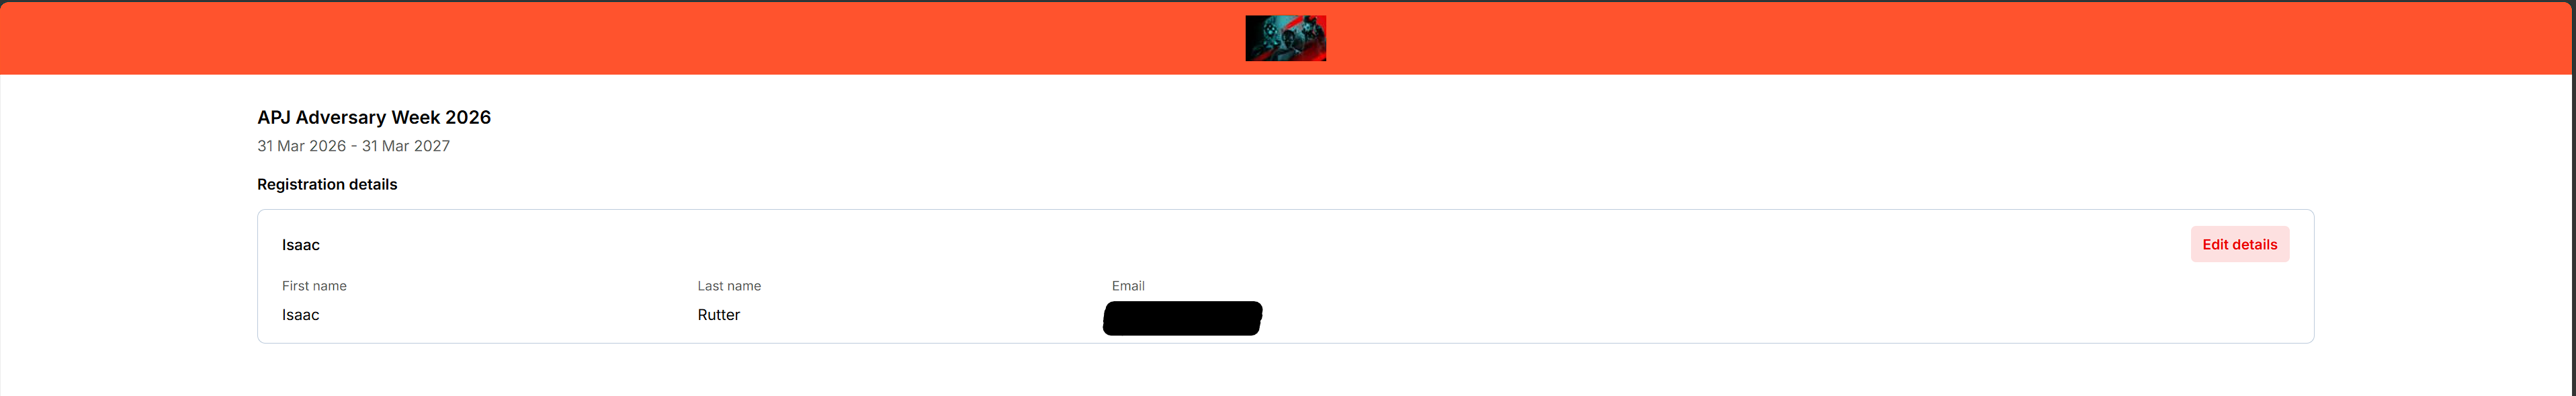
\includegraphics{registration_details.png}

\hypertarget{identity-based-attacks}{%
\subsection{Identity-Based Attacks}\label{identity-based-attacks}}

Although I signed up for five of these seminars, I was only able to
participate in one due to scheduling conflicts. Specifically, I
participated in the Identity-Based Attacks seminar since this was the
one which aligned with the unit content the most and the one I had the
most interest in.
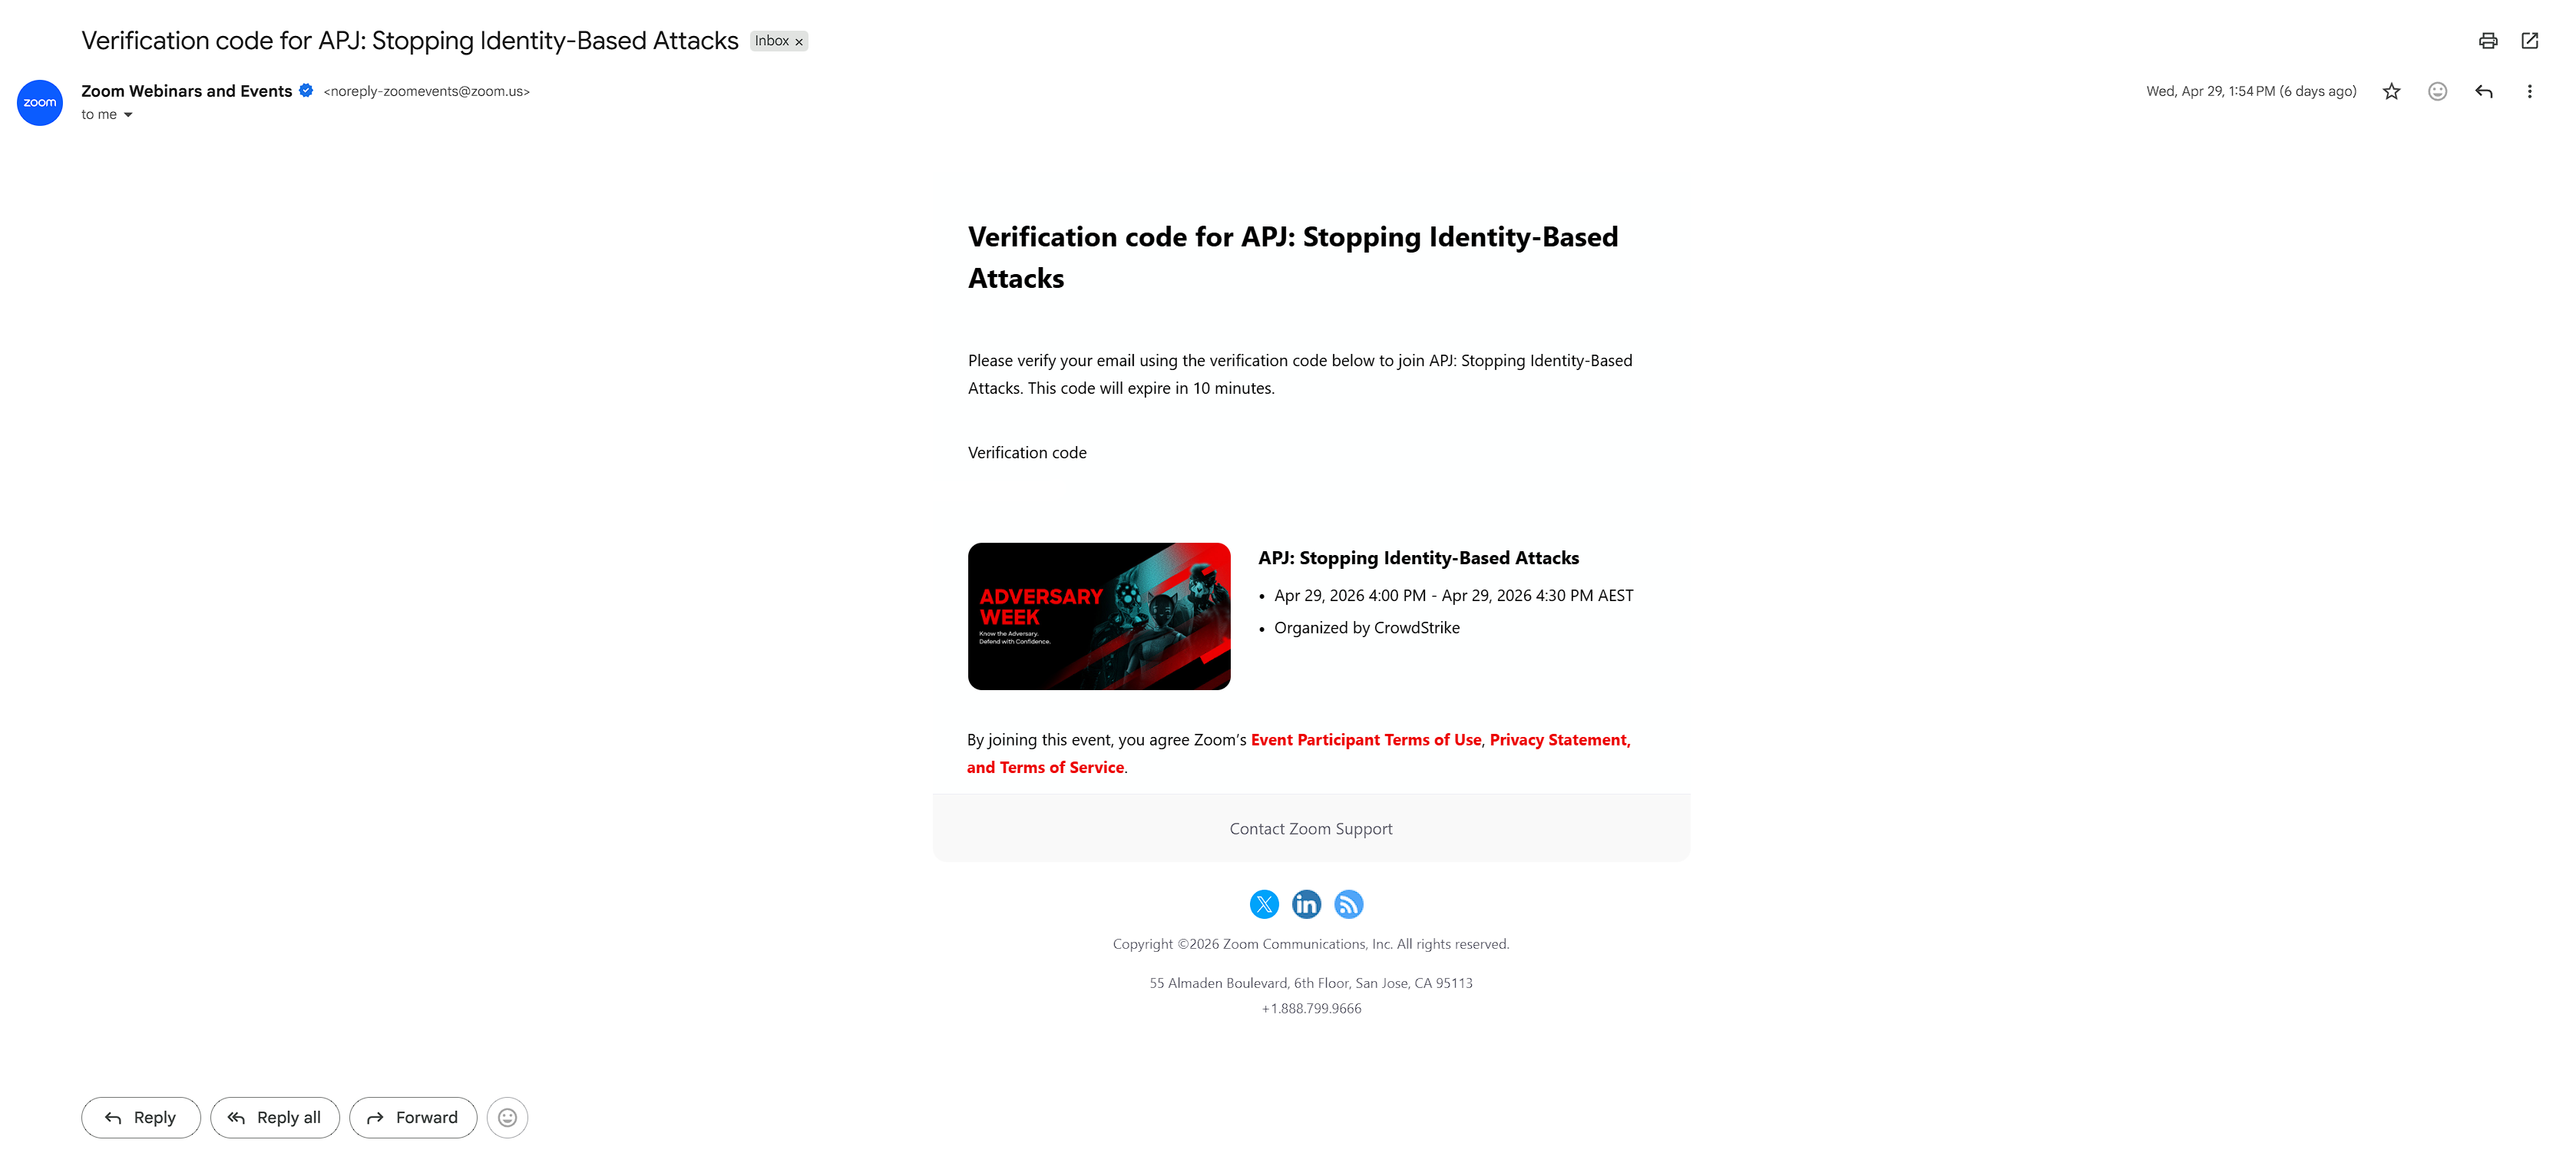
\includegraphics{Identity-Based Attacks/attendance_verification.png}

This seminar, as the name suggests, focused on identity-based attacks
and how to prevent them. It began with an insight into the evolution of
identity-based attacks, and made note of how IAM systems were designed
for control rather than security (and hence have no security/risk
alerts). 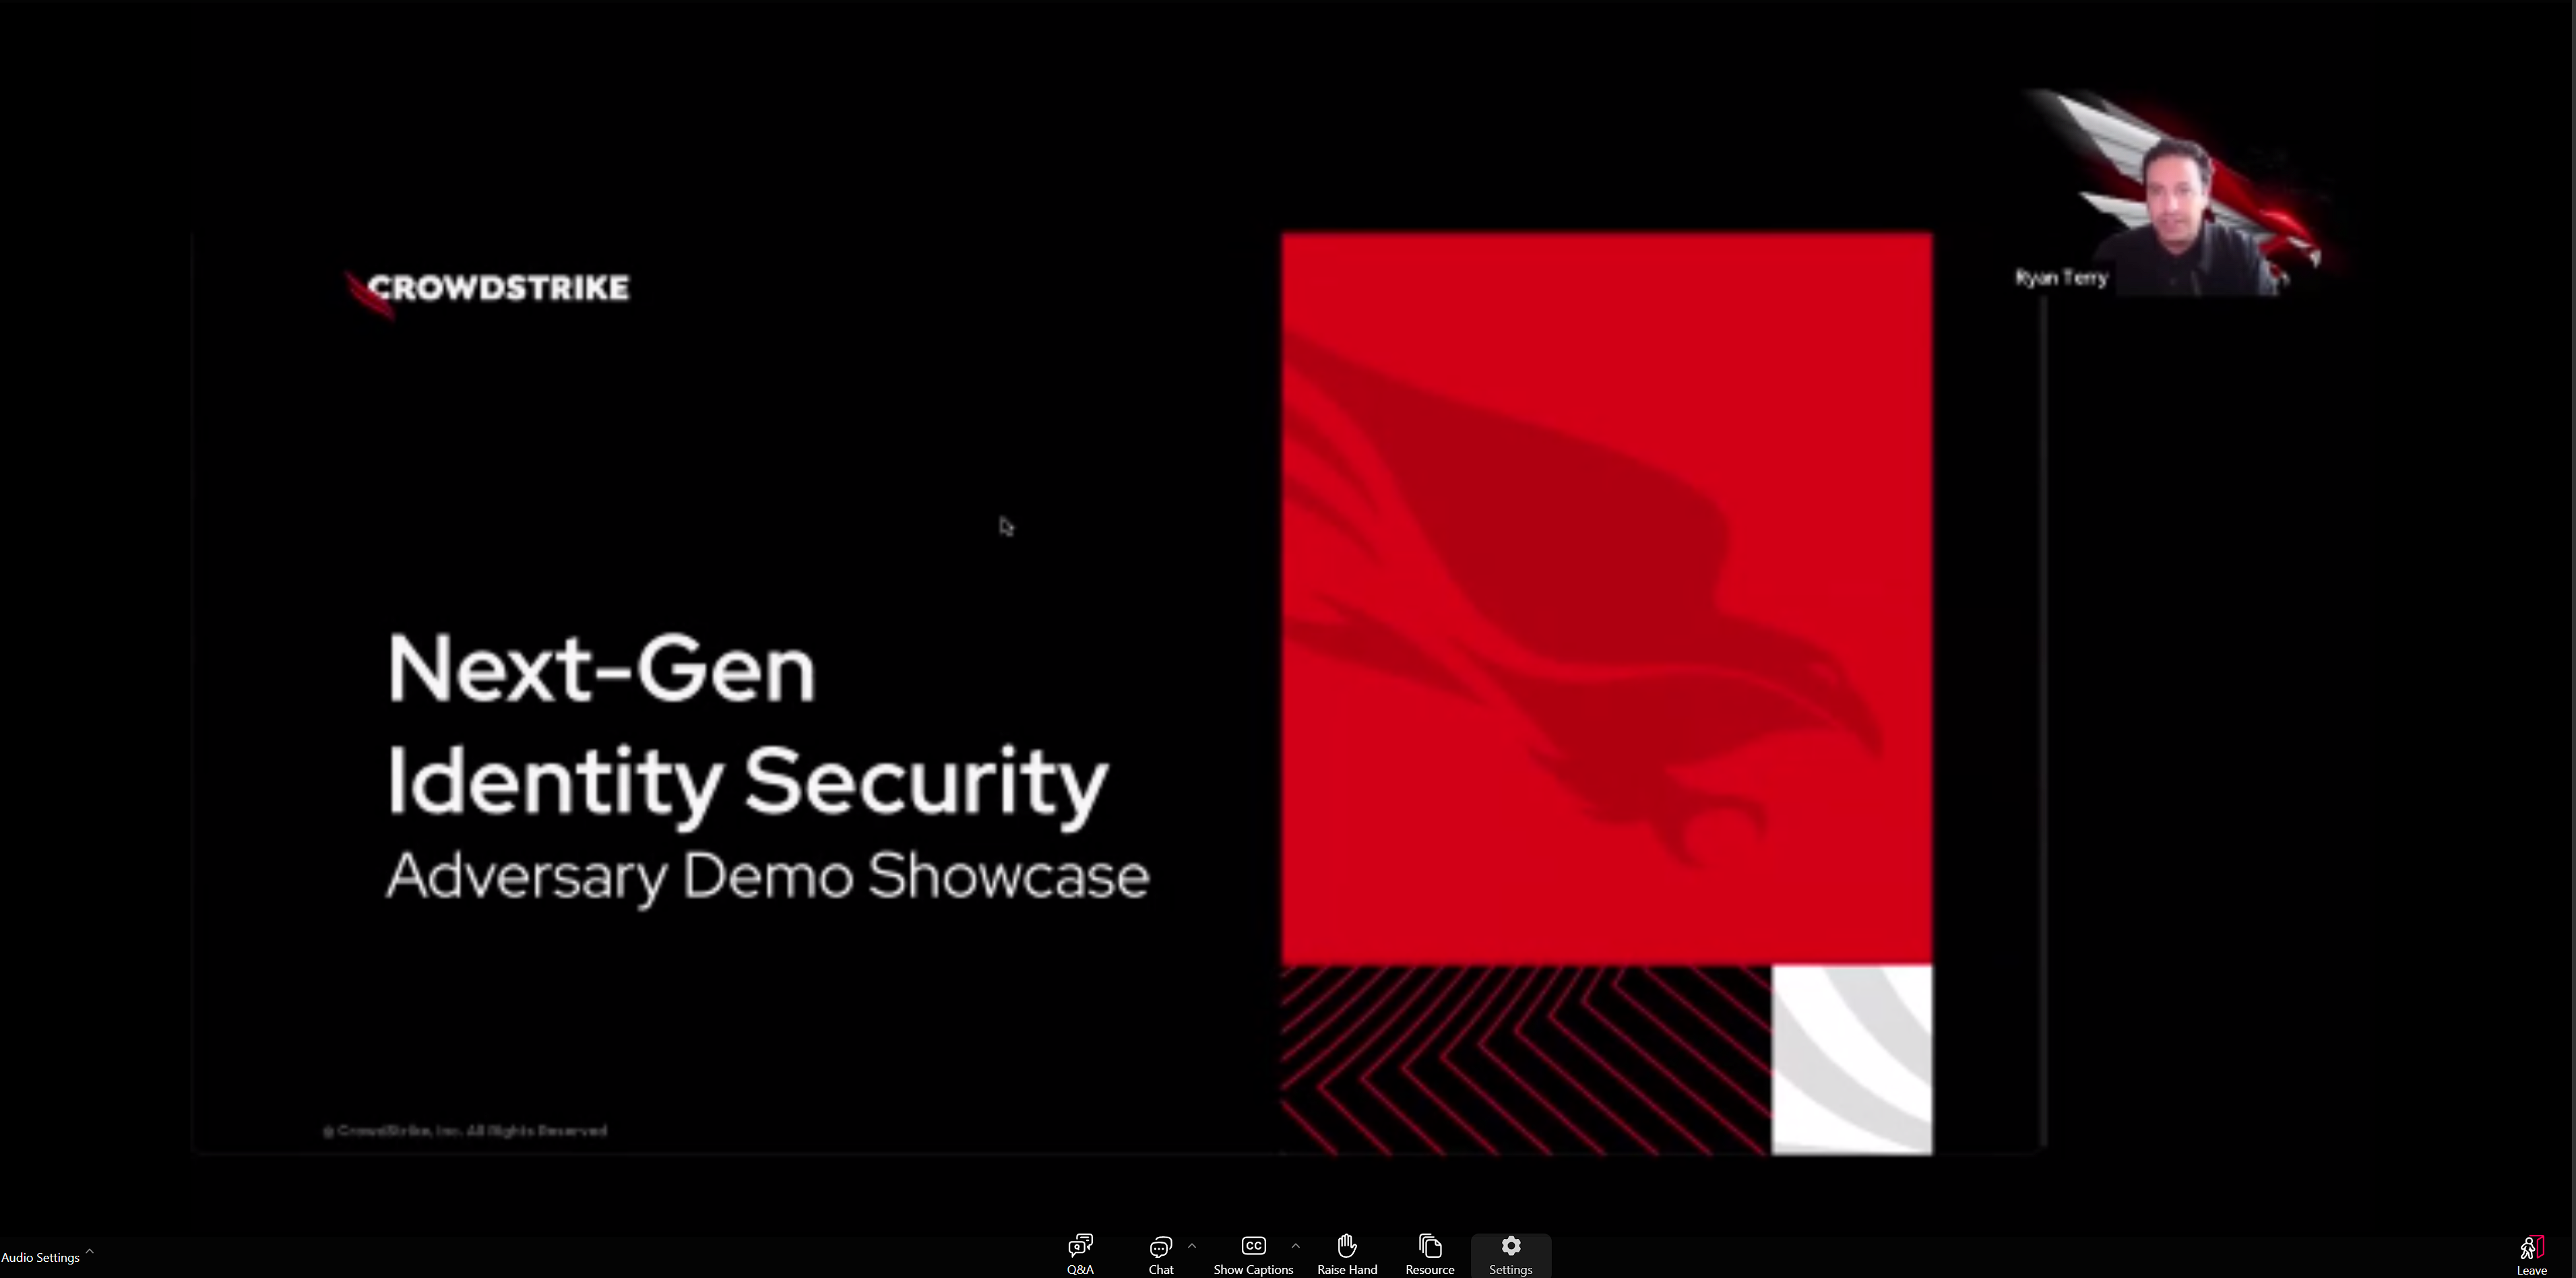
\includegraphics{Identity-Based Attacks/intro.png}

The seminar then moved on to insights into modern adversaries, including
their motivations, landscape, and threat intelligence.
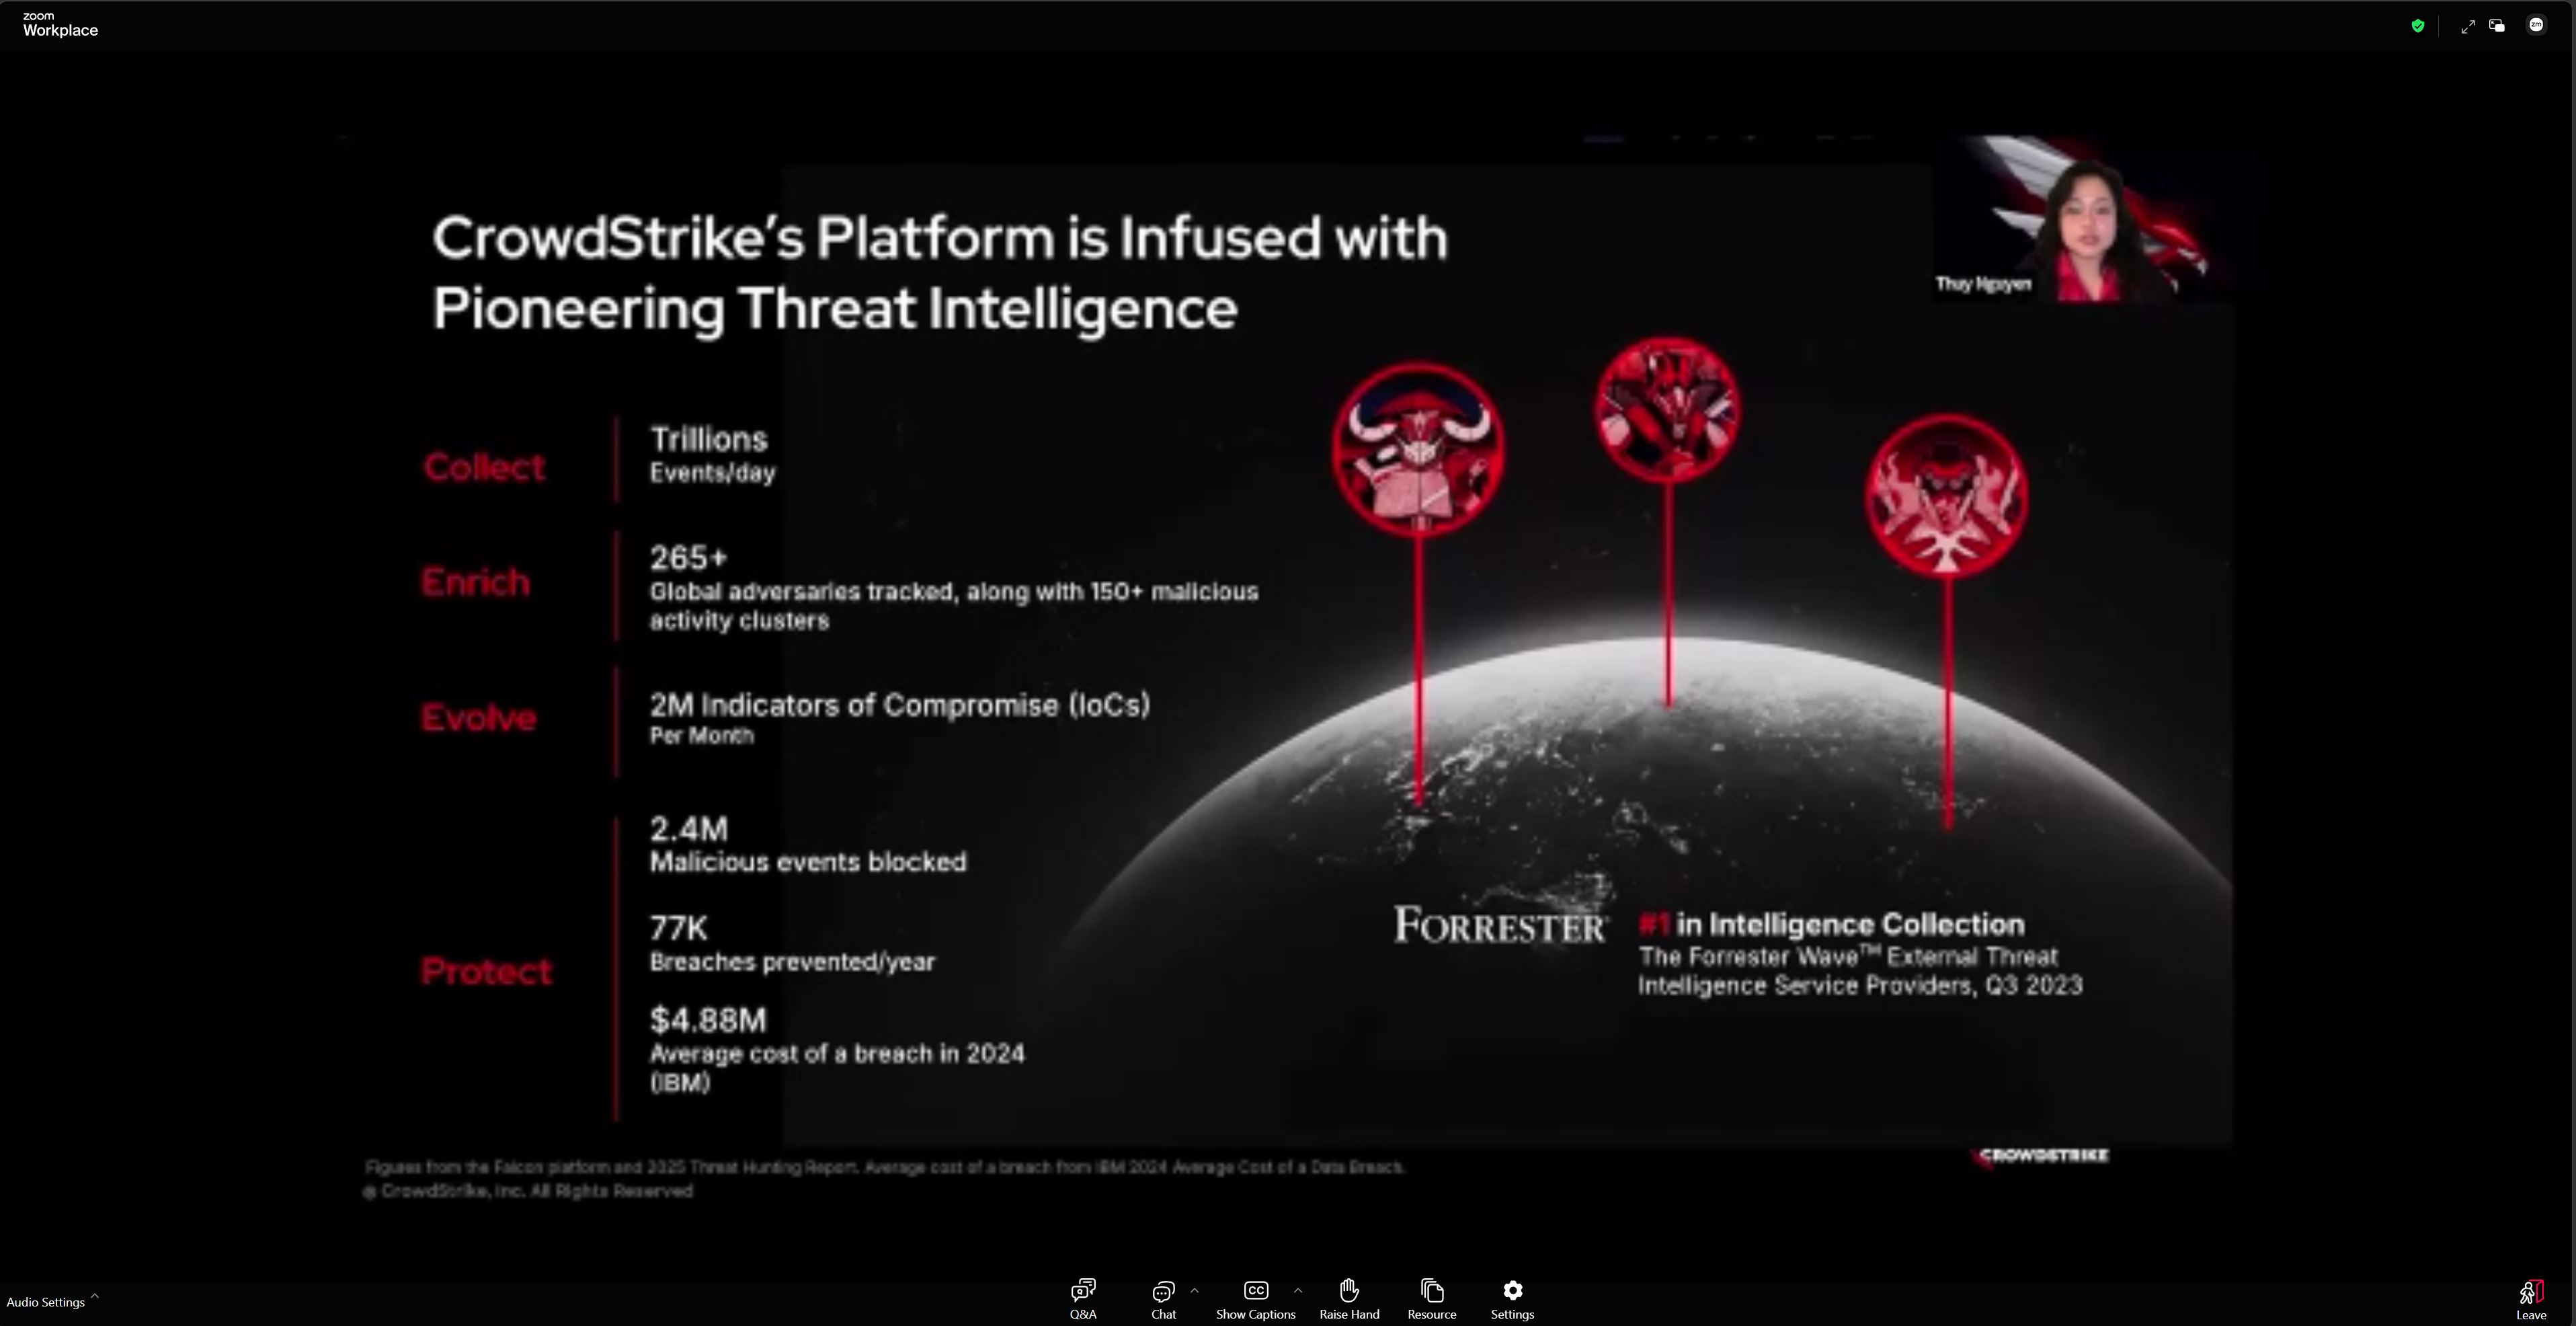
\includegraphics{Identity-Based Attacks/threat_intelligence.png}

The seminar then featured a brief demo of CrowdStrike's Falcon platform,
and how it can be used to protect against threats in real-time across
all of an organisation's applications with native integration. Finally,
the seminar ended with a Q\&A session where they answered some of the
questions that other participants had during the seminar.

\hypertarget{conclusion}{%
\section{Conclusion}\label{conclusion}}

Overall, the event provided valuable insight into the modern security
landscape surrounding identity-based attacks and exposed me to threats
and defence mechanisms that I was previously unaware of. The
demonstration of how these attacks can be mitigated was particularly
useful, as it showcased some of the modern tools and techniques used to
defend against constantly evolving threats.
